\documentclass[border=4pt]{standalone}
\usepackage{fontspec}
\setmainfont{TeX Gyre Heros}
\usepackage{tikz}
\usetikzlibrary{positioning,arrows.meta}
\definecolor{ink}{HTML}{1F1E1D}\definecolor{muted}{HTML}{6B6B6B}\definecolor{fill}{HTML}{EFEFEE}\definecolor{accent}{HTML}{3F6C8F}
\newcommand{\sub}{\fontsize{6.5bp}{8bp}\selectfont\color{muted}}
\begin{document}
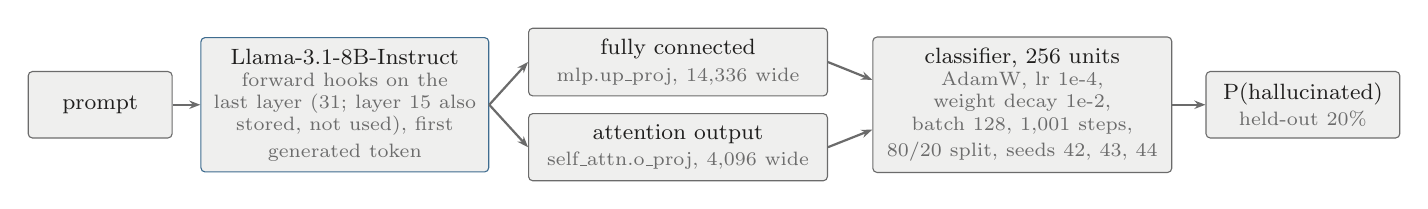
\begin{tikzpicture}[font=\fontsize{8bp}{9.5bp}\selectfont\color{ink},
 box/.style={draw=muted,fill=fill,rounded corners=1.5pt,align=center,inner sep=4pt,minimum height=24pt,text width=#1},
 arr/.style={-{Stealth[length=4pt]},draw=muted,thick}]
\node[box=44pt] (q) {prompt};
\node[box=96pt,right=10pt of q,draw=accent] (ll) {Llama-3.1-8B-Instruct\\{\sub forward hooks on the\\last layer (31; layer 15 also\\stored, not used), first\\generated token}};
\node[box=100pt,above right=0pt and 14pt of ll.east,anchor=south west,yshift=3pt] (fc) {fully connected\\{\sub mlp.up\_proj, 14,336 wide}};
\node[box=100pt,below right=0pt and 14pt of ll.east,anchor=north west,yshift=-3pt] (at) {attention output\\{\sub self\_attn.o\_proj, 4,096 wide}};
\node[box=100pt,anchor=west] (cl) at ([xshift=16pt]fc.east |- ll.east) {classifier, 256 units\\{\sub AdamW, lr 1e-4, weight decay 1e-2,\\batch 128, 1,001 steps,\\80/20 split, seeds 42, 43, 44}};
\node[box=62pt,right=12pt of cl] (pr) {P(hallucinated)\\{\sub held-out 20\%}};
\draw[arr](q)--(ll);\draw[arr](ll.east)--(fc.west);\draw[arr](ll.east)--(at.west);
\draw[arr](fc.east)--([yshift=9pt]cl.west);\draw[arr](at.east)--([yshift=-9pt]cl.west);
\draw[arr](cl)--(pr);
\end{tikzpicture}
\end{document}
